% !TEX TS-program = pdflatex
% !TEX encoding = UTF-8 Unicode

% This is a simple template for a LaTeX document using the "article" class.
% See "book", "report", "letter" for other types of document.

\documentclass[11pt]{article} % use larger type; default would be 10pt

\usepackage[utf8]{inputenc} % set input encoding (not needed with XeLaTeX)
\usepackage[T1]{fontenc}
\usepackage{times}

\usepackage{graphicx} % support the \includegraphics command and options

\usepackage[francais]{babel}

\usepackage{listings}

\usepackage{url}

\usepackage{rotating}

\usepackage[a4paper]{geometry}


\date{\today}

\title{Rapport Travaux Pratiques : \\Programmation par Contraintes\\ - TP 1 : \\\textbf{Découverte de la bibliothèque de contraintes à domaines finis}}
\author{Nicolas Desfeux\\Aurélien Texier}
\begin{document}
\lstset{language=Prolog,breaklines=true,numbers=left,basicstyle=\footnotesize ,numberstyle=\footnotesize}
\maketitle
\tableofcontents
\newpage
\section{De Prolog à Prolog+ic}
\subsection{Des contraintes sur les arbres}
\paragraph{Question 1.1}
L'objectif est  ici de définir un prédicat permettant d'effectuer un choix parmi des ensembles. Voici le code de nos prédicats, ainsi que les tests associés.
\lstinputlisting[caption="Prédicat choixCouleur"]{choixCouleur}
\paragraph{Question 1.2}
Prolog parcourt les branches de l'arbre des possibilités et il coupe les branches qui ne
s'unifient pas avec les contraintes.\\
Il s'arrête quand il a parcouru toutes les possibilités, et donc il génère toutes les solutions possibles,
toutes celles qui remplissent les contraintes.
\subsection{Prolog ne comprend pas les Maths (mais il a une bonnne calculatrice)}
\paragraph{Question 1.3}
Voici le code du prédicat isBetween : 
\lstinputlisting[caption="Prédicat isBetween"]{isBetween}
\paragraph{Question 1.4}
Voici le code du prédicat commande, et les tests associés : 
\lstinputlisting[caption="Prédicat commande"]{commande}
Le test de commande permet de valider le fonctionnement de \textit{isBetween/2}.
\paragraph{Question 1.5}
Le temps de réponse n'est pas négligeable puisqu'il est de 7.73 secondes.\\
En utilisant la trace de l'exécution, on constate que l'on est ici dans un contexte de "Generate and Test",
qui est dans ce cas beaucoup plus coûteux en temps.\\
Il génère les solutions qui sont dans les intervalles données (il y en a beaucoup !),
puis il teste celles qui remplissent la condition >=.\\
Comme on peut le constater dans le dessin de l'arbre de recherche Porlog ci-joint (figure \ref{arbre1} page \pageref{arbre1}), Prolog rencontre
dans son arbre de recherche beaucoup d'échecs puisqu'il génère tout, et c'est cela la cause de la perte de
beaucoup de temps d'exécution.
\begin{figure}
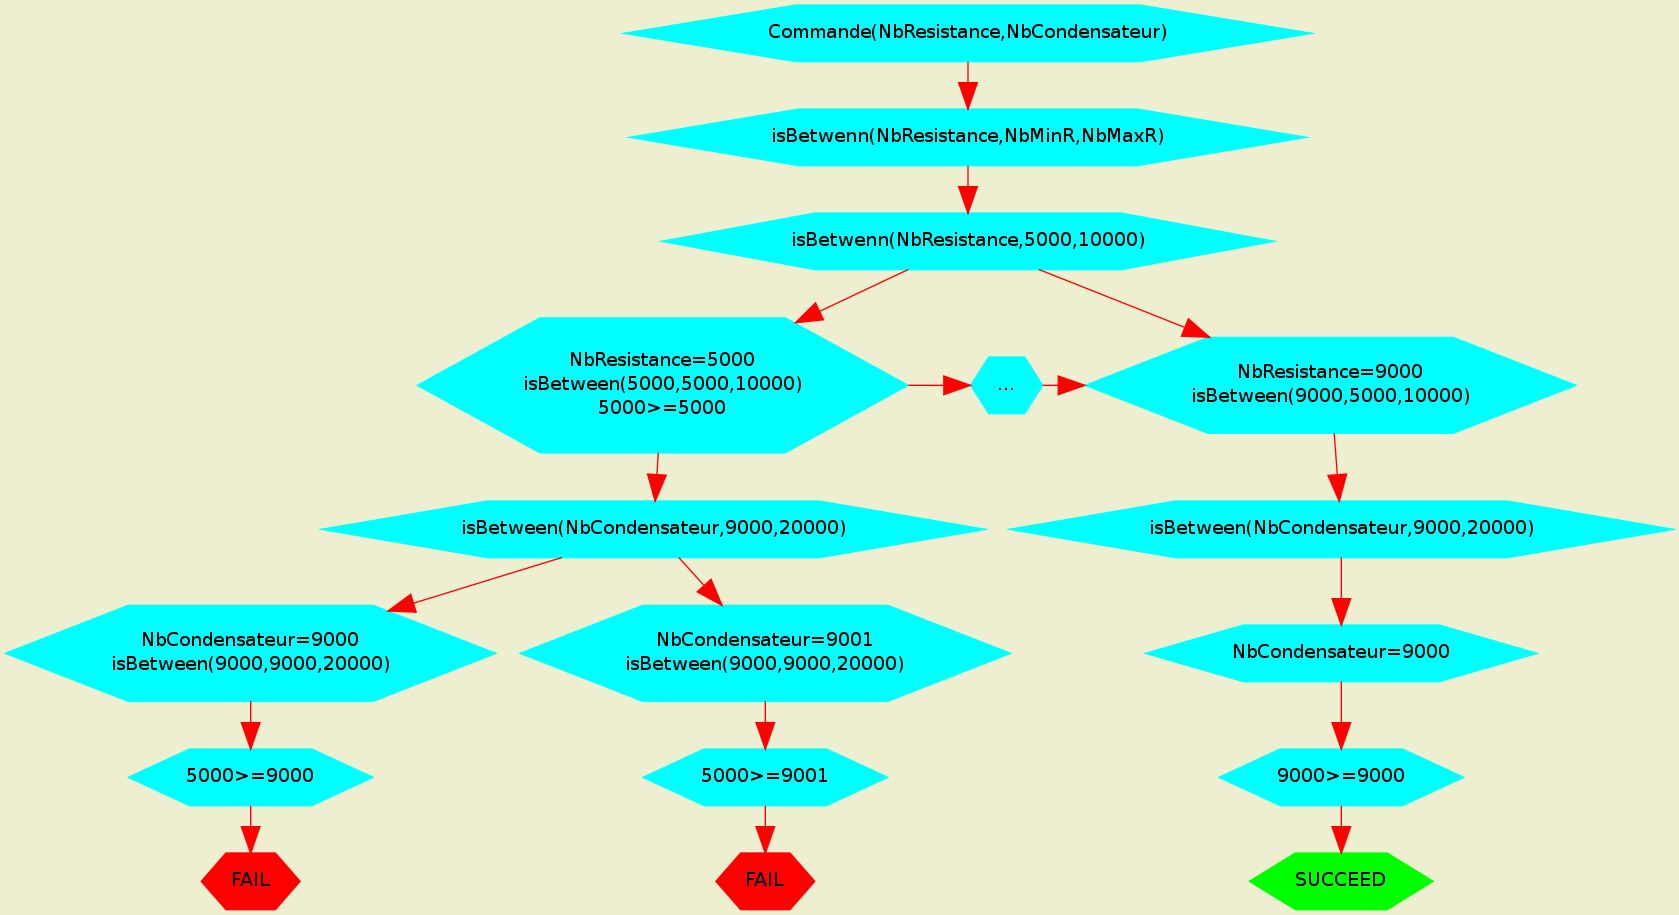
\includegraphics[width=15cm]{tp1.png}
\caption{\label{arbre1}Arbre Prolog 1}
\end{figure}
\paragraph{Question 1.6}
On réitère l'essai mais en mettant le prédicat >= avant le isBetween.\\
Nous sommes ici dans un cas de figure de "Constraints and Generate"
On voit alors ici que Prolog ne peut pas trouver de solution car pour remplir la condition
sur le >=, il y a une infinité de solutions puisqu'il ne sait pas encore dans quel intervalle travailler.
Donc il nous répond qu'il y a une faute d'instanciation.
Dans le cas d'avant, le isBetween permettait de lui donner un nombre fini de solutions pour les deux variables,
et après il pouvait alors trouver les solutions qui remplissaient le >=.
Nous sommes pour le commandeBis dans un cas de figure de "Generate and Test", puisqu'il génère les solutions sans
regarder ce qu'il a après comme condition.
\subsection{Le solveur ic à la rescousse}
\paragraph{Question 1.7}
Nous implémentons ici le prédicat \textit{commande2/2} en remplaçant isBetween par des commandes ic.
\lstinputlisting[caption="prédicat Commande"]{commande2}
Ici, la réponse d'eclipse est que les intervalles réponses pour les 2 variables sont
[9000,10000].
\paragraph{Question 1.8}
Nous implémentons ici le prédicat \textit{commande3/2}, basé sur \textit{commande2/2}, en utilisant \textit{labeling}.
\lstinputlisting[caption="prédicat Commande"]{commande3}
Ici, on voit clairement que le temps de réponse est vraiment plus rapide (moins d'un centième de seconde),
et ceci est dû au fait que le labeling, à savoir le solveur ic, regarde toutes les contraintes avant de
générer les solutions. Ce qui signifie qu'ici, il a réduit à l'avance les intervalles de solutions minimales
avant de générer les réponses. C'est un gain de temps énorme pour le cas ici présent puisque l'arbre de recherche
de Prolog (figure \ref{arbre2}, page \pageref{arbre2}) ne rencontre jamais d'échecs car il se construit dans les bonnes intervalles.
\begin{figure}
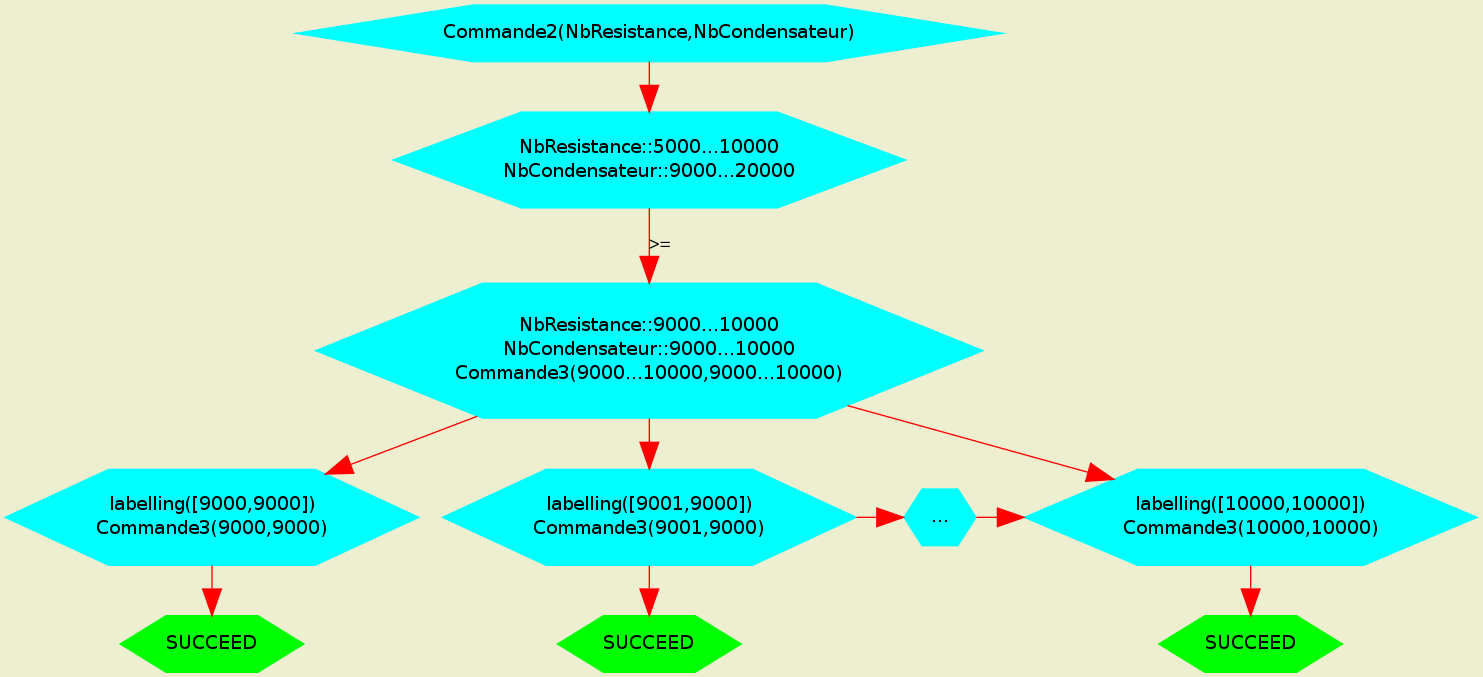
\includegraphics[width=15cm]{tp1-1.png}

\caption{\label{arbre2}Arbre Prolog 2}
\end{figure}

\newpage
\section{Zoologie}
Pour répondre aux questions, nous avons implémenté le prédicat \textit{chapie/4}.
\lstinputlisting[caption="Prédicat chapie"]{chapie}
\paragraph{Question 1.9}
Il faut donc 3 pies et 14 pattes pour totaliser 5 têtes et deux chats.
\lstinputlisting[caption="Prédicat chapie - test"]{chapie1}
\paragraph{Question 1.10}
Ici, il y a donc une infinité de solutions. La première donnée par le solveur est
{0,0,0,0} puis {1,1,6,2}, etc.
\lstinputlisting[caption="Prédicat chapie - test"]{chapie2}

\section{Le "OU" en contraintes}
\paragraph{Question 1.11}

 
Les deux prédicats ont ici exactement la même attitude pour ce cas de figure.
\lstinputlisting[caption="Prédicat vabs - vabs2"]{vabs}

Ici, seul la première version du prédicat donne les deux résultats corrects attendus.
\paragraph{Question 1.12}
Nous n'afficherons pas les tests car ils prennent de la place.
Pour la première version du prédicat, cela donne bien toutes les solutions possibles,
d'abord pour les X positifs puis pour les négatifs.
Pour la deuxième version, le prédicat donne d'abord les solution {0,0}, puis les solutions
négatives pour X, puis les positives.

\paragraph{Question 1.13}
Définition du prédicat \textit{faitListe/4} : 
\lstinputlisting[caption="Prédicat faitListe"]{faitListe}
Les résultats du test sont logiques, puisque 1 n'est pas entre Min et Max !

\paragraph{Question 1.14}
Définition du prédicat \textit{suite/1} :
\lstinputlisting[caption="Prédicat suite"]{suite}

\paragraph{Question 1.15}
Cette requête permet de visualiser les suites formées par le prédicat avec les 2 premiers
éléments de cette suite compris entre 1 et 10. Effectivement, il semble y avoir périodicité entre le premier
et le dixième élément (et donc une période de 9).
\lstinputlisting[caption="Réquête"]{q15}
Requête vérifiant que la suite est périodique de période 9
(vérifie qu'il n'existe aucune suite L ayant son premier et son dixième élément différents avec les deux premiers
éléments de la suite compris entre 1 et 10).\\
Prolog répond bien non à cette requête. On réitère alors avec les deux premiers éléments de la suite compris
entre 1 et 100.\\
La réponse est toujours non.\\
Enfin, on essaie avec les deux premiers éléments de la suite compris entre 1 et 1000.
Après plus d'une minute, Prolog répond toujours non.\\\\
Pour conclure, dans le prédicat suite, on remarquera que l'on est dans de la propagation et non du backtracking
puisque l'on construit la suite au fur et à mesure du parcourt de l'arbre à l'exécution.
Il n'y a donc pas besoin de faire appel au prédicat labeling.
\newpage

\section{Code Complet, avec tests}
\lstinputlisting[caption="test"]{tp1}
\end{document}
